\documentclass[12pt]{article}

\usepackage{Sweave}
\begin{document}
\title{Homework 4}
\author{Qin Qian}
\Sconcordance{concordance:3rd.tex:3rd.Rnw:%
1 2 1 1 0 10 1 1 2 1 0 4 1 3 0 1 2 4 1 1 2 1 0 1 41 43 0 1 2 3 1 1 3 9 %
0 1 1 11 0 1 2 15 0 3 1 1 3 1 0 2 1 1 2 1 0 4 1 3 0 1 2 3 1 1 32 34 0 1 %
2 3 1 1 4 106 0 1 2 2 1 1 7 6 0 1 1 26 0 1 2 2 1 1 2 4 0 1 2 2 1 1 3 2 %
0 1 1 3 0 1 2 1 1 2 2 3 1 1 21 23 0 1 2 1 1 1 2 1 0 2 1 9 0 1 2}

\maketitle
\vspace{-1cm}

\section{Load packages and extract expression values from .CEL files}
Load packages:
\begin{Schunk}
\begin{Sinput}
> library(affy)
> library(limma)
> library(AnnotationDbi)
> library(hgu133plus2hsentrezgcdf)      
> library(hgu133plus2hsentrezg.db)  
\end{Sinput}
\end{Schunk}

\begin{quotation}
RNA expression analysis workflow written with function rna.workflow
\end{quotation}

\begin{Schunk}
\begin{Sinput}
> setwd("~/Desktop/2012_fall_training/3rd/GSE10437/")
> rna.workflow <- function(pat, pd, method, cdf){
+   # rna expression process workflow
+   # pat for files suffix
+   # pd for phenotype data
+   # cdf for annotation files
+   files <- dir(pattern=pat)
+   pd <- read.AnnotatedDataFrame(pd,header=T,
+                                row.names=1, sep="", as.is=T)
+   data.affy <- read.affybatch(filenames=files, phenoData=pd)
+   
+   #data.affy <- ReadAffy()
+   data.affy@cdfName <- cdf
+   
+   if (method=="rma") {
+     data.result <- rma(data.affy)
+     data.expr <- exprs(data.result)
+     data.expr.PA <- ""
+   }
+   if (method=="mas"){
+     data.result <- mas5(data.affy)
+     data.expr <- exprs(data.result)   # expression value
+     # use log 2 instead of e
+     data.expr <- log2(data.expr)
+     data.expr.PA <- exprs(mas5calls(data.affy)) # expression pattern, see help
+   }
+ 
+   # ajust ids
+   genes_t = matrix(rownames(data.expr))
+   genes.refseq=apply(genes_t, 1, function(x) sub("_at", "", x))
+   orig.refseq=rownames(data.expr)
+ 
+   rownames(data.expr) <- genes.refseq
+ 
+   if (all(data.expr.PA!="")) {
+     data<-list(refseq=genes.refseq, expr=data.expr, eset=data.result, PA=data.expr.PA, orig=orig.refseq)
+   }
+   else{
+     data<-list(refseq=genes.refseq, expr=data.expr, eset=data.result,orig=orig.refseq)
+   }
+   return(data)
+ }
\end{Sinput}
\end{Schunk}

\section{Call function rna.workflow, Remove absent genes with mas5.0call method}
remove genes without expression, that is to say, with four A

\begin{Schunk}
\begin{Sinput}
> rna.expression.rma <- rna.workflow(".CEL", "GSE10437.txt",
+                                    "rma", "hgu133plus2hsentrezgcdf") 
\end{Sinput}
\begin{Soutput}
Background correcting
Normalizing
Calculating Expression
\end{Soutput}
\begin{Sinput}
> head(rna.expression.rma$expr)
\end{Sinput}
\begin{Soutput}
                M0       T0      M18      T18
1         6.397041 6.470414 5.811688 6.111480
10        3.952028 3.859540 3.788875 3.987352
100       9.104029 9.071492 7.118385 7.115066
1000      4.931831 4.703695 4.666662 5.066794
10000     5.471414 5.920217 4.703620 4.827628
100009676 4.703420 4.981382 5.563516 5.131319
\end{Soutput}
\begin{Sinput}
> rna.expression.mas5 <- rna.workflow(".CEL", "GSE10437.txt",
+                                     "mas", "hgu133plus2hsentrezgcdf") 
\end{Sinput}
\begin{Soutput}
background correction: mas 
PM/MM correction : mas 
expression values: mas 
background correcting...done.
18989 ids to be processed
|                    |
|####################|
Getting probe level data...
Computing p-values
Making P/M/A Calls
\end{Soutput}
\begin{Sinput}
> write.table(rna.expression.mas5$expr, file="rna_mas5.txt", sep="\t", quote=F)
> entrezid <- featureNames(rna.expression.mas5$eset)
> affy.control <- grep("^A", entrezid, perl=T)
> # remove affymetrix control probes
> rna.expression.mas5$expr <- rna.expression.mas5$expr[-affy.control,]
> rna.expression.mas5$PA <- rna.expression.mas5$PA[-affy.control,]
> rna.expression.mas5$orig <- rna.expression.mas5$orig[-affy.control]
> # remove Absent gene and missing genes
> rna.expression.mas5$expr <- rna.expression.mas5$expr[-affy.control,]
> rna.absent <- apply(rna.expression.mas5$PA, 1, paste, collapse="")
> rna.absent.index <- grep("AAAA", rna.absent)
> rna.expression.mas5$expr <- rna.expression.mas5$expr[-rna.absent.index,]
> rna.expression.mas5$orig <- rna.expression.mas5$orig[-rna.absent.index]
\end{Sinput}
\end{Schunk}

\section{Use limma to analyze differential gene expression with Group means}
Write a function called rna.diff

\begin{Schunk}
\begin{Sinput}
> rna.diff <- function(expr="", ref="", eset="", control, treat, method){
+   if (method=="foldT"){
+     # fold change and T-test
+     foldchange=apply(expr, 1, function(x) mean(x[treat])-mean(x[control]))
+     T.p.value=apply(expr, 1, 
+                     function(x) t.test(x[treat], x[control], var.equal=T)$p.value)
+     #fdr=p.adjust(T.p.value, method="BH") # BH, Bonferroni, fdr
+     fdr = T.p.value
+ 
+     # genes
+     genes.up = expr[which(fdr<0.05 & foldchange>0)]
+ 
+     genes.down = expr[which(fdr<0.05 & foldchange<0)]
+     genes.id = c(which(fdr<0.05 & foldchange>0), which(fdr<0.05 & foldchange<0))    
+     return(expr[genes.id,])
+   }
+   # limma group means
+   if (method=="gm"){
+     gm.design<-model.matrix(~ 0+factor(c(1,1,2,2)))
+     colnames(gm.design) <- c("control","treat")
+ #    gm.design = cbind(control = control, treat = treat)
+     print(gm.design)
+     gm.fit = lmFit(expr, gm.design)
+     print(gm.fit)
+     gm.matrix = makeContrasts(CvsT = control-treat, levels=gm.design)
+     gm.fit = contrasts.fit(gm.fit, gm.matrix)
+     gm.fit = eBayes(gm.fit)
+     diff.expr <- topTable(gm.fit, p.value=0.05, lfc=2, number=length(expr[,1]), adjust.method="BH") 
+     return(diff.expr)
+   }
+ }
\end{Sinput}
\end{Schunk}

Call function rna.diff to extract differential expression genes
toptable

\begin{Schunk}
\begin{Sinput}
> diff.result.gm <- rna.diff(rna.expression.mas5$expr, rna.expression.mas5$refseq,
+                            rna.expression.mas5$eset,
+                            c(1,1,0,0), c(0,0,1,1),"gm")
\end{Sinput}
\begin{Soutput}
  control treat
1       1     0
2       1     0
3       0     1
4       0     1
attr(,"assign")
[1] 1 1
attr(,"contrasts")
attr(,"contrasts")$"factor(c(1, 1, 2, 2))"
[1] "contr.treatment"

An object of class "MArrayLM"
$coefficients
            control     treat
1          7.944705  7.073364
100       10.535276  8.278494
10000      8.098391  6.905428
100009676  6.405914  7.258350
10001     10.541649 10.686756
11534 more rows ...

$rank
[1] 2

$assign
[1] 1 1

$qr
$qr
     control      treat
1 -1.4142136  0.0000000
2  0.7071068 -1.4142136
3  0.0000000  0.7071068
4  0.0000000  0.7071068
attr(,"assign")
[1] 1 1
attr(,"contrasts")
attr(,"contrasts")$"factor(c(1, 1, 2, 2))"
[1] "contr.treatment"


$qraux
[1] 1.707107 1.000000

$pivot
[1] 1 2

$tol
[1] 1e-07

$rank
[1] 2


$df.residual
[1] 2 2 2 2 2
11534 more elements ...

$sigma
        1       100     10000 100009676     10001 
0.3334615 0.2320161 0.2454466 0.7822903 0.2229627 
11534 more elements ...

$cov.coefficients
        control treat
control     0.5   0.0
treat       0.0   0.5

$stdev.unscaled
            control     treat
1         0.7071068 0.7071068
100       0.7071068 0.7071068
10000     0.7071068 0.7071068
100009676 0.7071068 0.7071068
10001     0.7071068 0.7071068
11534 more rows ...

$pivot
[1] 1 2

$genes
[1] "1"         "100"       "10000"     "100009676" "10001"    
11534 more rows ...

$method
[1] "ls"

$design
  control treat
1       1     0
2       1     0
3       0     1
4       0     1
attr(,"assign")
[1] 1 1
attr(,"contrasts")
attr(,"contrasts")$"factor(c(1, 1, 2, 2))"
[1] "contr.treatment"
\end{Soutput}
\end{Schunk}

\section{Extract chromosome annotations from hgu133plus2entrezg.db}
Get whole annotations
\begin{Schunk}
\begin{Sinput}
> myAnnot <- data.frame(
+     ID=sapply(contents(hgu133plus2hsentrezgENTREZID), paste, collapse=", "), 
+     SYMBOL=sapply(contents(hgu133plus2hsentrezgSYMBOL), paste, collapse=", "), 
+     DESC=sapply(contents(hgu133plus2hsentrezgGENENAME), paste, collapse=", "),
+     CHR=sapply(contents(hgu133plus2hsentrezgCHR), paste, collapse=", ")
+ )
> head(myAnnot)
\end{Sinput}
\begin{Soutput}
                    ID       SYMBOL
100009676_at 100009676 LOC100009676
10000_at         10000         AKT3
10001_at         10001         MED6
10002_at         10002        NR2E3
10003_at         10003      NAALAD2
100048912_at 100048912   CDKN2B-AS1
                                                                                DESC
100009676_at                                            uncharacterized LOC100009676
10000_at     v-akt murine thymoma viral oncogene homolog 3 (protein kinase B, gamma)
10001_at                                                  mediator complex subunit 6
10002_at                             nuclear receptor subfamily 2, group E, member 3
10003_at                              N-acetylated alpha-linked acidic dipeptidase 2
100048912_at                                                  CDKN2B antisense RNA 1
             CHR
100009676_at   3
10000_at       1
10001_at      14
10002_at      15
10003_at      11
100048912_at   9
\end{Soutput}
\end{Schunk}

use merge to get exact match between differential expression genes and
whole annotations
\begin{Schunk}
\begin{Sinput}
> merge.diffwithanno <- merge(myAnnot[,c(1,4)],diff.result.gm[,c(1,3)],all=F)
\end{Sinput}
\end{Schunk}

use table to get the statistics of every chromosome genes

\begin{Schunk}
\begin{Sinput}
> chrNames=c("Y","X", "22","21","20","19","18","17","16","15","14","13",
+            "12","11","10","9","8","7","6","5","4","3","2","1")
> chr.statstable <- table(merge.diffwithanno$CHR)[chrNames]
\end{Sinput}
\end{Schunk}

\section{Draw barplot for differential expressed genes number on every chromosome}
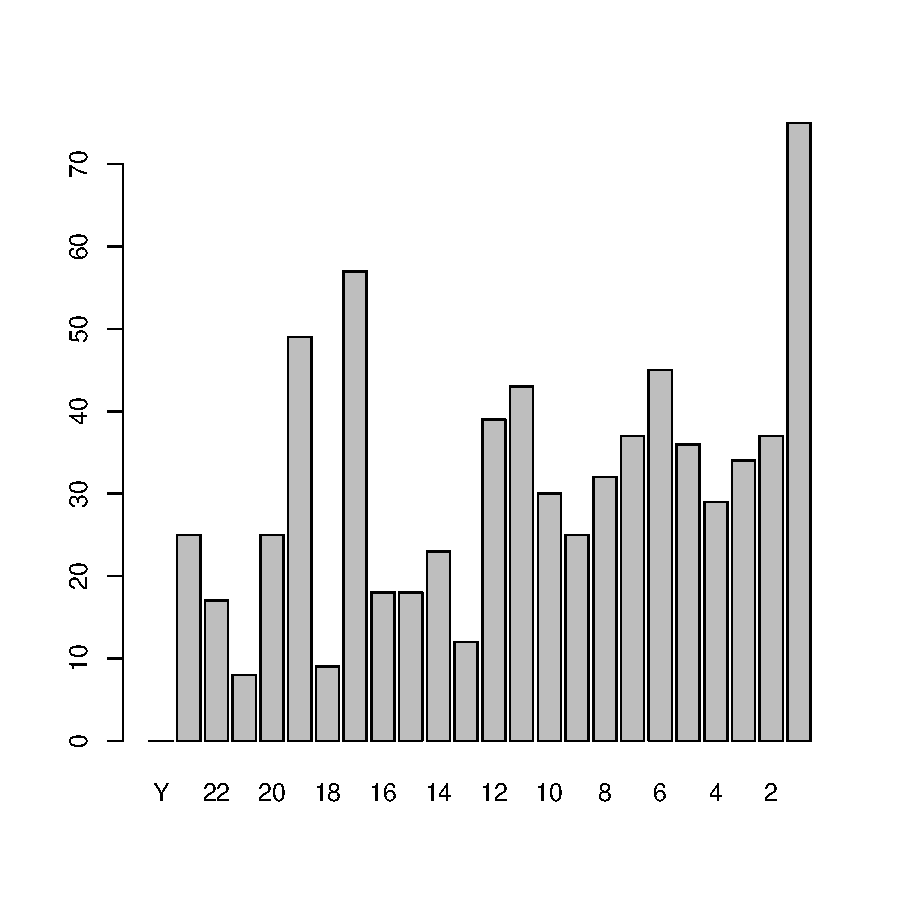
\includegraphics{3rd-009}

\section{Fisher test on chromosome 1 between differential
  expressed and non differential expressed genes}
write a function called chr.number.test on each chromosome
\begin{Schunk}
\begin{Sinput}
> chr.number.test <- function(diffgenes,chrdata,n) {
+   # chrdata = for differentiatial expressed genes on chromosomes 
+   # n denotes which chromosomes
+ 
+   chrn.diff.len <- length(grep(paste("^", n, "$", sep=""),chrdata[,2],perl=T))
+   print(chrn.diff.len)
+   CHR=sapply(contents(hgu133plus2hsentrezgCHR), paste, collapse=", ")
+   chrn.len <- length(grep(paste("^", n, "$", sep=""),CHR,perl=T))
+   nonchrn.diff <- length(diffgenes) - chrn.diff.len
+   nonchrn.len <- length(CHR) - chrn.len  
+   chrn.nondiff.len <- chrn.len - chrn.diff.len
+   nonchrn.nondiff <- nonchrn.len - nonchrn.diff
+   # matrix for fisher test
+   chrndiff.fisher <- matrix(c(chrn.diff.len, chrn.nondiff.len, nonchrn.diff, nonchrn.nondiff),
+                             nrow=2, dimnames=list(chr=c(paste("chr", n), paste("nonchr",n)), diff=c("diff","nondiff")))
+   cat("greater side p.value", fisher.test(chrndiff.fisher,alternative="greater")$p.value,"\n")
+   cat("less side p.value", fisher.test(chrndiff.fisher,alternative="less")$p.value,"\n")
+   cat("two sided p.value",fisher.test(chrndiff.fisher,alternative="two.sided")$p.value,"\n")
+   return(chrndiff.fisher)
+ }
\end{Sinput}
\end{Schunk}
call function on differential expressed genes on chromosome 1st
chr for all differential expressed genes chromosome annotations
\begin{Schunk}
\begin{Sinput}
> entrez.diff <- rna.expression.mas5$orig[as.numeric(rownames(diff.result.gm))]
> chr <- toTable(hgu133plus2hsentrezgCHR[entrez.diff])
> diff.fisher<-chr.number.test(entrez.diff, chr, 1)
\end{Sinput}
\begin{Soutput}
[1] 75
greater side p.value 0.3655605 
less side p.value 0.6803715 
two sided p.value 0.7037721 
\end{Soutput}
\end{Schunk}
\end{document}
